\let\negmedspace\undefined
\let\negthickspace\undefined
\documentclass[a4,12pt,onecolumn]{IEEEtran}
\usepackage{amsmath,amssymb,amsfonts,amsthm}
\usepackage{algorithmic}
\usepackage{graphicx}
\usepackage{textcomp}
\usepackage{xcolor}
\usepackage{txfonts}
\usepackage{listings}
\usepackage{enumitem}
\usepackage{mathtools}
\usepackage{gensymb}
\usepackage[breaklinks=true]{hyperref}
\usepackage{tkz-euclide}
\usepackage{listings}
\usepackage{gvv}
\begin{document}
\title{
\Huge\textbf{ Analog Assignment}\\
\Huge\textbf{EE1205} Signals and Systems\\
}
\large\author{Kurre Vinay\\EE23BTECH11036}
\maketitle
\textbf{Question 11.9.3.8:}
 Two towers on top of two hills are $40$ km apart.This line joining them passes $50$ m above a hill halfway between the towers.What is the longest wavelength of radio waves,which can be sent between the towers without  appereciable diffraction effects?\\
\solution
\begin{table}[ht!]
 \begin{center}
\begin{tabular}{|c|c|c|}
   \hline
   variable&value&description  \\
   \hline
   d & $40$ km& distance between the towers\\
   \hline
   a & $50$ m & size of aperture \\
   \hline
   $\lambda$ &$\frac{a^2}{Z_f} $ & longest wavelength of radio wave\\
   \hline
   $Z_f$ &20 Km &Fresnel distance, $Z_f$ is the half of the distance between the towers \\
   \hline
\end{tabular}
\caption{\large{Input Parameters}}
\end{center}
\end{table}
\begin{align}
Z_f&=\frac{a^2}{\lambda}\\
\lambda &= \frac{a^2}{Z_f}\\
&=\frac{50^2}{20000}\\
&= 125 \times 10^{-3} \text{m}\\
&= 12.5 \text{cm}\end{align}
the longest wavelength of radio waves, which can be sent in between the towers without considerable diffraction effects is 12.5 cm 
\begin{figure}[ht!]
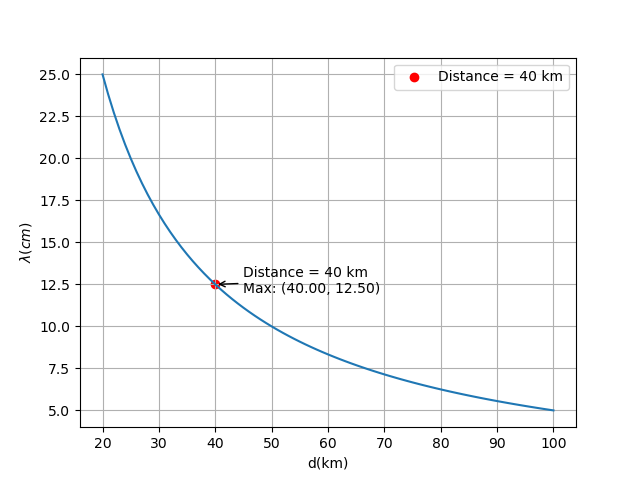
\includegraphics[width=\columnwidth]{figs/fig2.png}
\caption{THE GRAPH BETWEEN THE MAXIMUM WAVELENGTH($\lambda$) Vs DISTANCE BETWEEN THE TOWERS(d)}
\end{figure}
\end{document}
